\documentclass{article}

\usepackage{graphicx}
\usepackage{tikz}
\usepackage{tikzsymbols}
\usetikzlibrary{calc,patterns,shapes.geometric}
\pagestyle{empty}
\usepackage[margin=0pt]{geometry}
\geometry{papersize={14in,12in}}

\def\centerarc[#1](#2)(#3:#4:#5){\draw[#1] ($(#2)+({#5*cos(#3)},{#5*sin(#3)})$) arc (#3:#4:#5);}

\begin{document}
	\begin{figure}
		\centering
		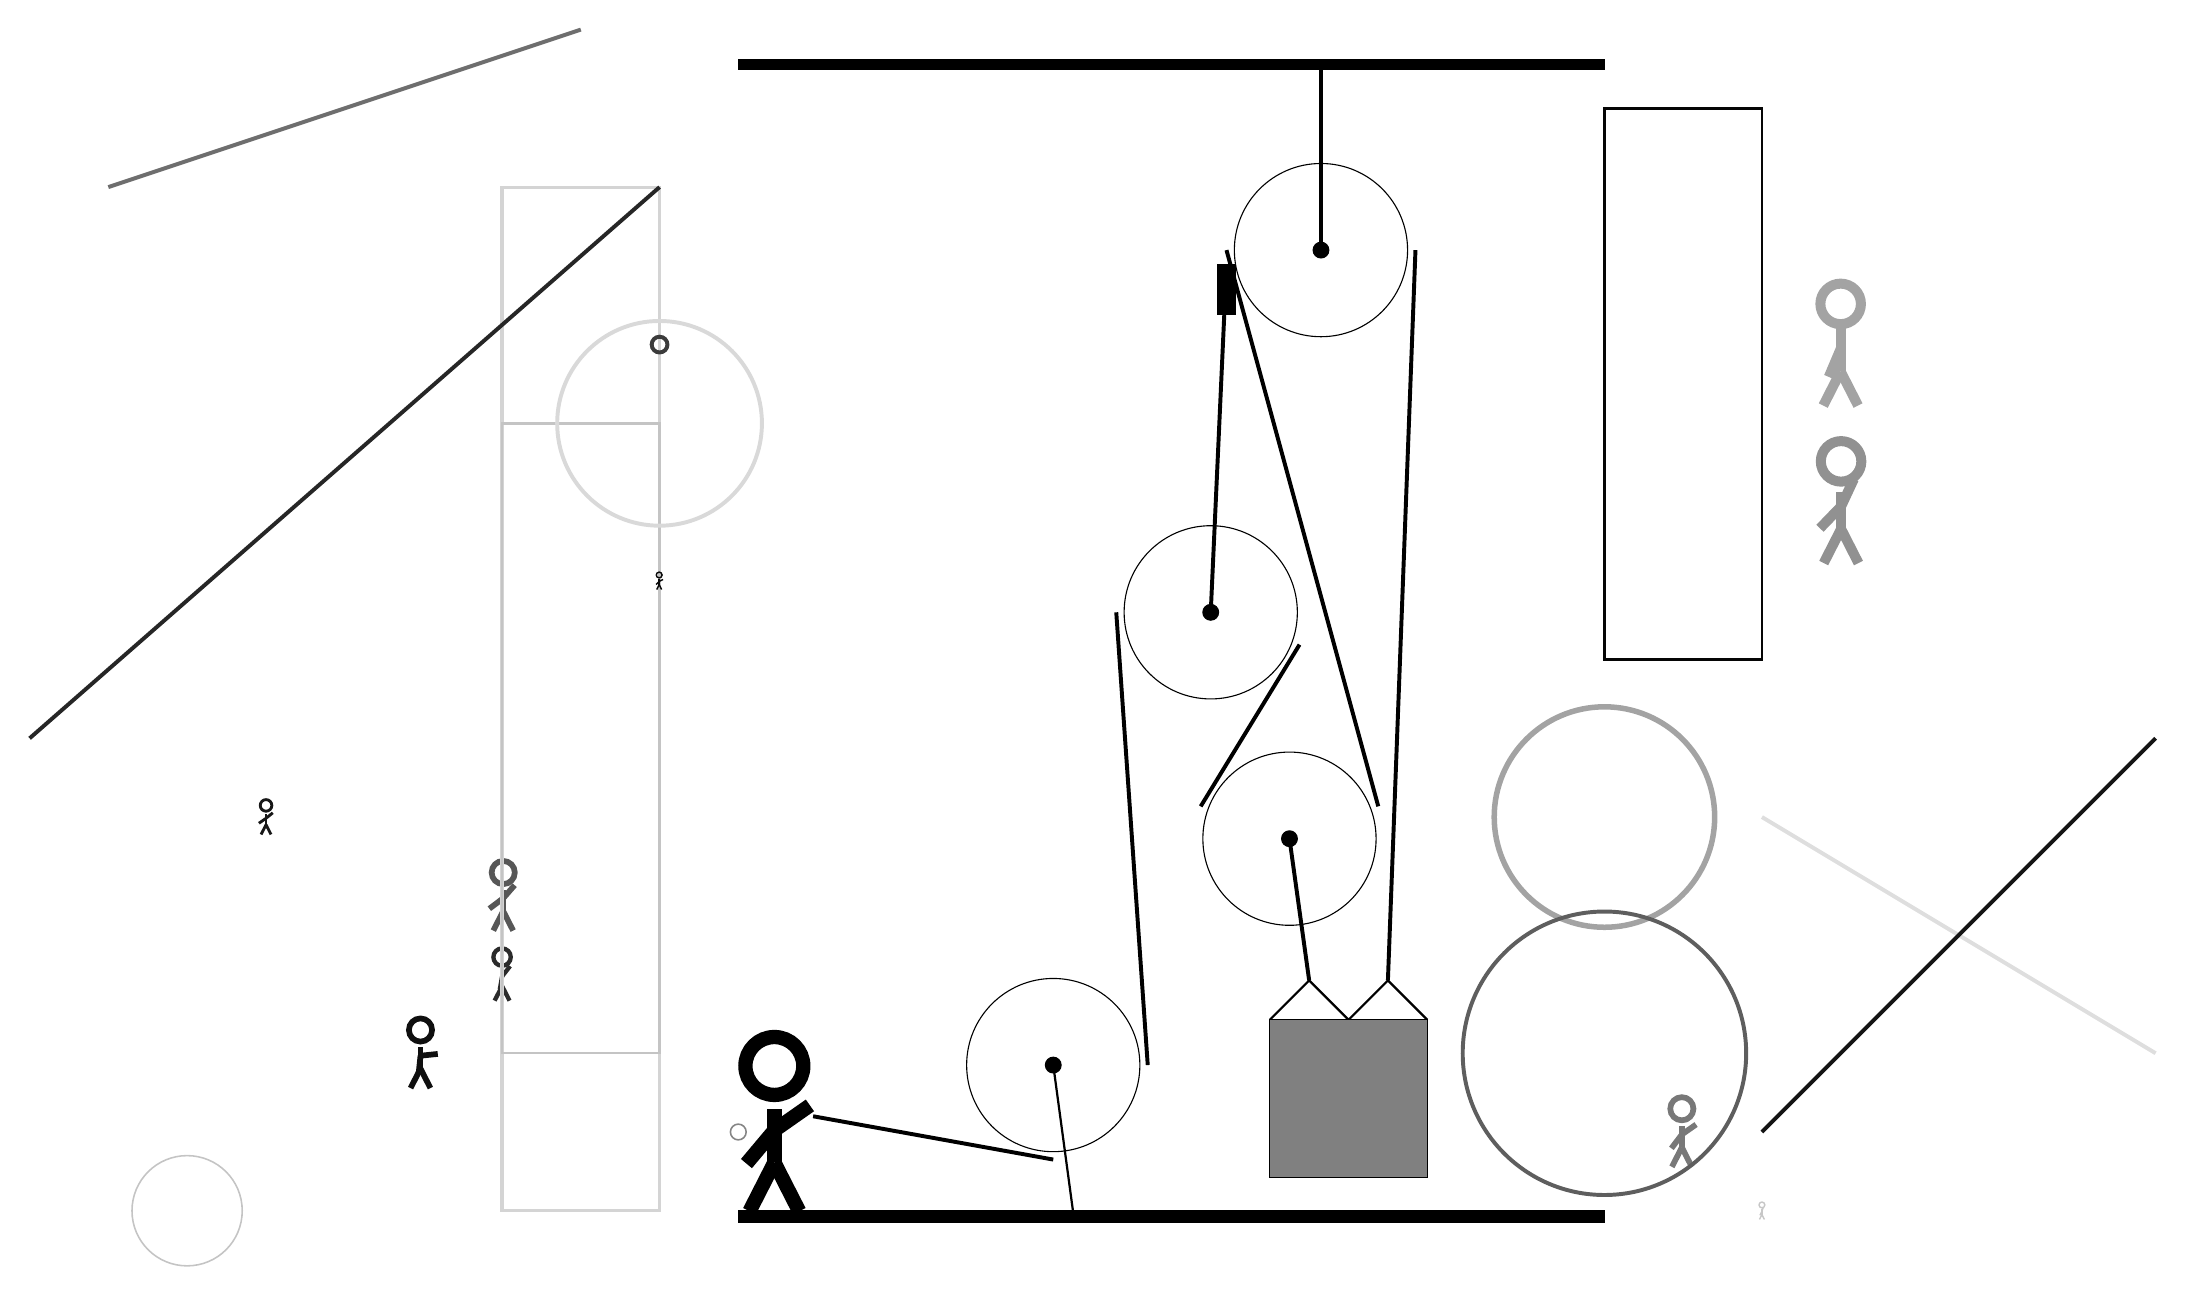
\begin{tikzpicture}
			%%%%% START %%%%%
			
			\draw[fill=black] (-6, 11.5) rectangle (5, 11.625);
			
			\draw (0, 4.6) circle (1.1);
			\draw[fill=black] (0, 4.6) circle (0.1);
			
			\draw (1, 1.725) circle (1.1);
			\draw[fill=black] (1, 1.725) circle (0.1);
			
			\draw (1.4, 9.2) circle (1.1);
			\draw[fill=black] (1.4, 9.2) circle (0.1);
			\draw[very thick] (1.4, 9.2) -- (1.4, 11.5);
			
			\draw (-2, -1.15) circle (1.1);
			\draw[fill=black] (-2, -1.15) circle (0.1);
			\draw[thick] (-2, -1.15) -- (-1.75, -3);
			
			
			\draw[thick]  (0.75, -0.575) -- (1.25, -0.075) -- (1.75, -0.575) -- (2.25, -0.075) -- (2.75, -0.575);
			\draw[fill=black!50] (0.75, -0.575) rectangle (2.75, -2.575);
			\draw[line width=0.5mm] (-5.05, -1.8) -- (-2, -2.35);
			\centerarc[line width=0.5mm](-2, -1.15)(270:360:1.2000000000000002);
			\draw[line width=0.5mm] (-0.8, -1.15) -- (-1.2, 4.6);
			\draw[line width=0.5mm] (0, 4.6) -- (0.2, 9.0);
			\draw[line width=0.5mm, fill=black](0.1, 8.4) rectangle (0.3, 9.0);
			\centerarc[line width=0.5mm](0, 4.6)(-20:180:1.2000000000000002);
			\draw[line width=0.5mm] (1.1276, 4.1896) -- (-0.1276, 2.1354);
			\centerarc[line width=0.5mm](1, 1.725)(160:380:1.2000000000000002);
			\draw[line width=0.5mm] (2.1276, 2.1354) -- (0.2, 9.2);
			\draw[line width=0.5mm](1, 1.725) -- (1.25, -0.075);
			\centerarc[line width=0.5mm](1.4, 9.2)(0:180:1.2000000000000002);
			\draw[line width=0.5mm] (2.6, 9.2) -- (2.25, -0.075);
			
			\node at (-5.5, -1.9) {\Strichmaxerl[10][50][35]};
			
			\node[line width=0.4mm, color=black!83] at (-9, 0) {\Strichmaxerl[3][80][52]};
			
			\draw [line width=0.2mm, color=black!23](-13, -3) circle (0.7);
			\draw[line width=0.5mm, color=black!13](7, 2) -- (12, -1);
			\node[line width=0.6mm, color=black!43] at (8, 6) {\Strichmaxerl[7][46][65]};
			\node[line width=0.7mm, color=black!66] at (-9, 1) {\Strichmaxerl[4][37][49]};
			\node[line width=0.5mm, color=black!22] at (7, -3) {\Strichmaxerl[1][63][72]};
			\draw[line width=0.5mm, color=black!57](-8, 12) -- (-14, 10);
			
			\draw[line width=0.4mm, color=black!17] (-7, 10) rectangle (-9, -3);
			\draw [line width=0.7mm, color=black!36](5, 2) circle (1.4);
			\draw[line width=0.3mm, color=black!98] (5, 4) rectangle (7, 11);
			\draw [line width=0.5mm, color=black!77](-7, 8) circle (0.1);
			\draw[line width=0.5mm, color=black!92](7, -2) -- (12, 3);
			\node[line width=0.5mm, color=black!94] at (-10, -1) {\Strichmaxerl[4][84][6]};
			\node[line width=0.5mm, color=black!36] at (8, 8) {\Strichmaxerl[7][67][90]};
			\draw [line width=0.2mm, color=black!48](-6, -2) circle (0.1);
			\node[line width=0.3mm, color=black!53] at (6, -2) {\Strichmaxerl[4][53][35]};
			
			\node[line width=0.3mm, color=black!91] at (-12, 2) {\Strichmaxerl[2][35][39]};
			\draw[line width=0.5mm, color=black!85](-7, 10) -- (-15, 3);
			\draw[line width=0.3mm, color=black!23] (-7, -1) rectangle (-9, 7);
			
			\draw [line width=0.5mm, color=black!63](5, -1) circle (1.8);
			\node[line width=0.2mm, color=black!96] at (-7, 5) {\Strichmaxerl[1][44][27]};
			
			\draw [line width=0.5mm, color=black!15](-7, 7) circle (1.3);
			
			
			\draw[fill=black] (-6, -3) rectangle (5, -3.15);
			
			%%%%% END %%%%%
		\end{tikzpicture}
	\end{figure}	
\end{document}